\documentclass[12pt,a4paper]{article}

\usepackage[T1,T2A]{fontenc}
\usepackage[utf8]{inputenc}
\usepackage[english, russian]{babel}
\usepackage{indentfirst}
\usepackage{misccorr}
\usepackage{graphicx}
\usepackage{amsmath}
\usepackage{graphicx}
\usepackage{float}
\usepackage[left=20mm,right=10mm, top=20mm,bottom=20mm,bindingoffset=0mm]{geometry}

\setlength{\parskip}{6pt}\graphicspath{{images/}}\DeclareGraphicsExtensions{.png}

\begin{document}

    \begin{titlepage}
        \begin{center}
            \large
            Санкт-Петербургский политехнический университет\\Петра Великого\\
            \vspace{0.5cm}
            Институт прикладной математики и механики\\
            \vspace{0.25cm}
            Кафедра «Прикладная математика»
            \vfill
            \textsc{\LARGE\textbf{Отчет по лабораторной работе №1}}\\[5mm]
            \Large
            по дисциплине\\"Математическая статистика"
        \end{center}
        \vfill
        \begin{tabular}{l p{175} l}
            Выполнила студентка\\группы 3630102/80201 && Деркаченко Анна Олеговна
            \vspace{0.25cm}
            \\Проверил\\доцент, к.ф.-м.н. && Баженов Александр Николаевич
        \end{tabular}
        \vfill
        \begin{center}
            Санкт-Петербург\\2021 г.
        \end{center}
    \end{titlepage}

\newpage
\begin{center}
    \tableofcontents
    \setcounter{page}{2}
\end{center}
\newpage
\begin{center}
    \listoffigures
\end{center}

\newpage
\section{Постановка задачи}
Даны распределения:
\begin{itemize}
    \item нормальное распределение $N(x,0,1)$
    \item распределение Коши $C(x,0,1)$
    \item распределение Лапласа $L(x,0,\frac{1}{\sqrt{2}})$
    \item распределение Пуассона $P(k,10)$
    \item равномерное распределение $U(x,-\sqrt{3},\sqrt{3})$
\end{itemize}

Необходимо:
\begin{enumerate}
    \item Сгенерировать выборки размером 10, 50 и 1000 элементов
    \item остроить на одном рисунке гистограмму и график плотности распределения
\end{enumerate}

\section{Теория}
\subsection{Распределения}
Плотности рассматриваемых распределений:
\begin{itemize}
		\item нормальное распределение
		    \begin{equation}
			    N(x,0,1)=\frac{1}{\sqrt{2\pi}}e^{-\frac{x^2}{2}}
			    \label{normal} 
			\end{equation}
		\item распределение Коши
		    \begin{equation}
				C(x,0,1)=\frac{1}{\pi}\frac{1}{x^2+1}
				\label{cauchy}
			\end{equation} 
		\item распределение Лапласа
		    \begin{equation}
				L(x,0,\frac{1}{\sqrt{2}})=\frac{1}{\sqrt{2}}e^{-\sqrt{2}|x|}
				\label{laplace} 
			\end{equation}
		\item распределение Пуассона
		    \begin{equation}
				P(k,10)=\frac{10^k}{k!}e^{-10}
				\label{poisson}
			\end{equation}
		\item равномерное распределение
		    \begin{equation}
				U(x,-\sqrt{3},\sqrt{3})=
				\begin{cases}
					\frac{1}{2\sqrt{3}},|x|\leq\sqrt{3}\\0,|x|>\sqrt{3}
				\end{cases}
				\label{uniform}
			\end{equation}
\end{itemize}

\subsection{Гистограмма}
\textit{Гистограмма} - функция, построенная на основе выборки из некоторого распределения и приближающая его плотность вероятности.

Гистограммы используются для визуализации данных в начале статистической обработки.

Графическое построение гистограммы:
\begin{enumerate}
    \item Множество значений, которые может принимать элемент выборки, разбивается на\\несколько интервалов
    \item Данные интервалы откладываются на горизонтальной оси
    \item Рисуется прямоугольник:
        \begin{itemize}
            \item с высотой, пропорциональной числу элементов выборки, попадающих в данный интервал, если интервалы одинаковы
            \item с площадью, пропорциональной числу элементов выборки, попадающих в данный интервал, если интервалы различны
        \end{itemize}
\end{enumerate}

\section{Реализация}
Реализация лабораторной работы проводилась на языке Python в среде разработки PyCharm c использованием дополнительных библиотек:
\begin{itemize}
    \item scipy
    \item numpy
    \item matplotlib
    \item math
\end{itemize}

Исходный код лабораторной работы размещен в GitHub-репозитории.

URL: https://github.com/derkanw/Mathstat/tree/main/lab1

\section {Результаты}
\begin{figure}[H]
    \centering
    \begin{tabular}{c c c}
        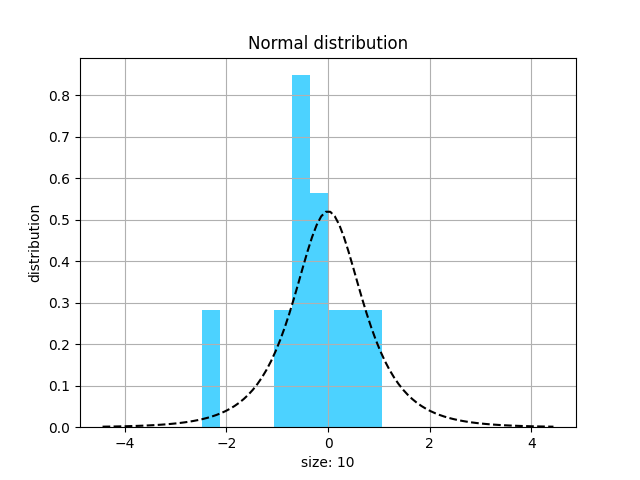
\includegraphics[height = 0.25\textheight, width = 0.31\textwidth]{Normal_10.png}
        & 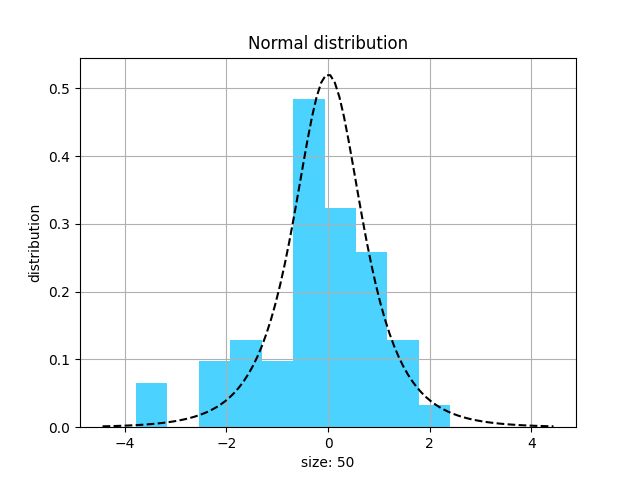
\includegraphics[height = 0.25\textheight, width = 0.31\textwidth]{Normal_50.png}
        & 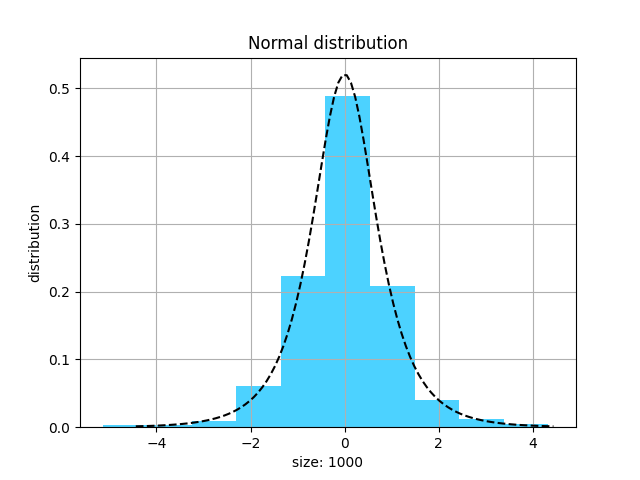
\includegraphics[height = 0.25\textheight, width = 0.31\textwidth]{Normal_1000.png}
    \end{tabular}
    \caption{Нормальное распределение \eqref{normal}}
    \label{fig:normal}
\end{figure}

\begin{figure}[H]
    \centering
    \begin{tabular}{c c c}
        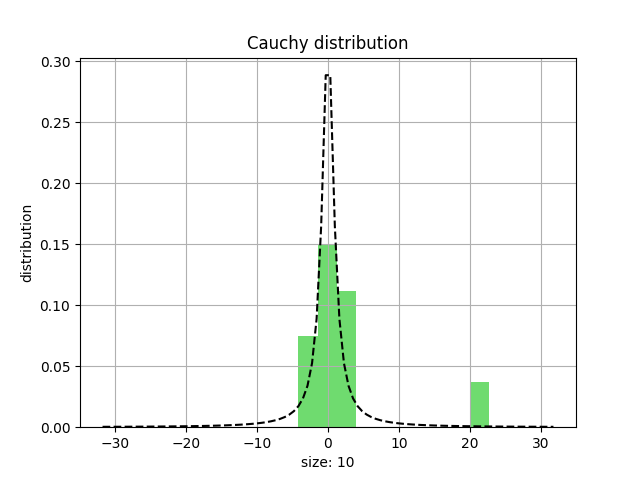
\includegraphics[height = 0.25\textheight, width = 0.31\textwidth]{Cauchy_10.png}
        & 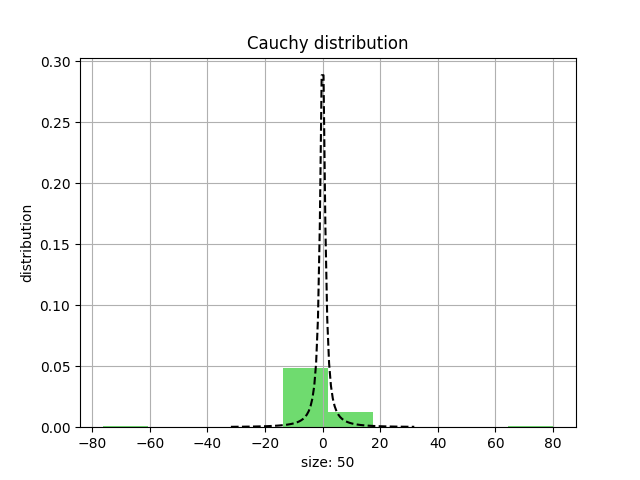
\includegraphics[height = 0.25\textheight, width = 0.31\textwidth]{Cauchy_50.png}
        & 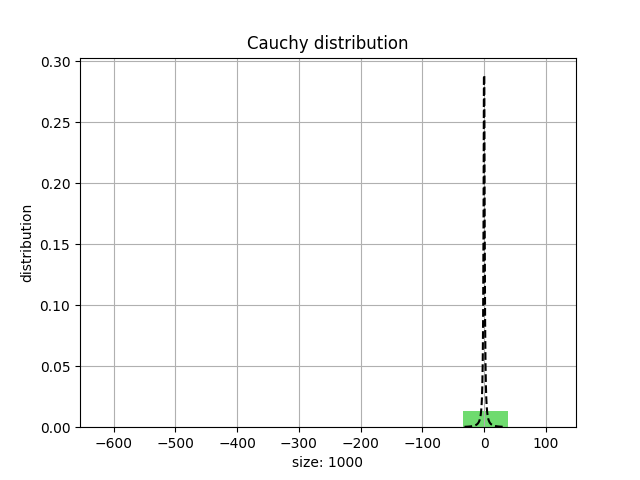
\includegraphics[height = 0.25\textheight, width = 0.31\textwidth]{Cauchy_1000.png}
    \end{tabular}
    \caption{Распределение Коши\eqref{cauchy}}
    \label{fig:cauchy}
\end{figure}

\begin{figure}[H]
    \centering
    \begin{tabular}{c c c}
        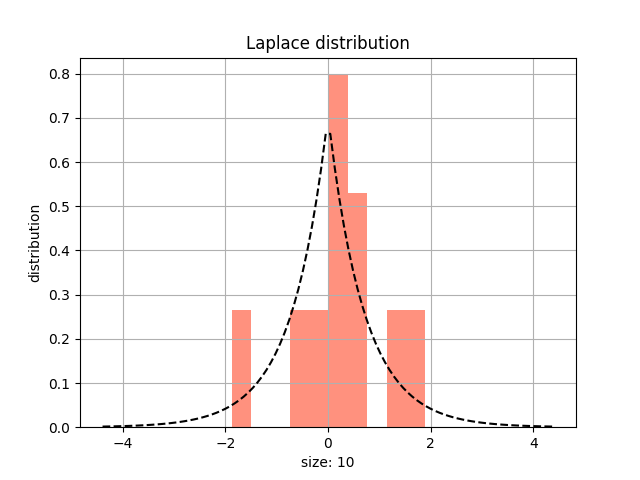
\includegraphics[height = 0.25\textheight, width = 0.31\textwidth]{Laplace_10.png}
        & 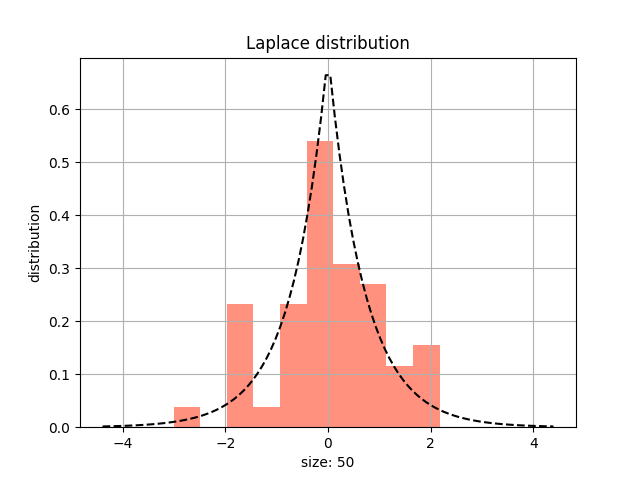
\includegraphics[height = 0.25\textheight, width = 0.31\textwidth]{Laplace_50.png}
        & 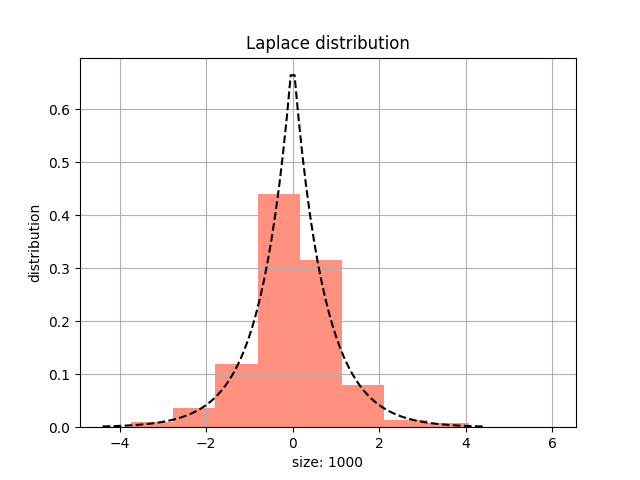
\includegraphics[height = 0.25\textheight, width = 0.31\textwidth]{Laplace_1000.png}
    \end{tabular}
    \caption{Распределение Лапласа \eqref{laplace}}
    \label{fig:laplace}
\end{figure}

\begin{figure}[H]
    \centering
    \begin{tabular}{c c c}
        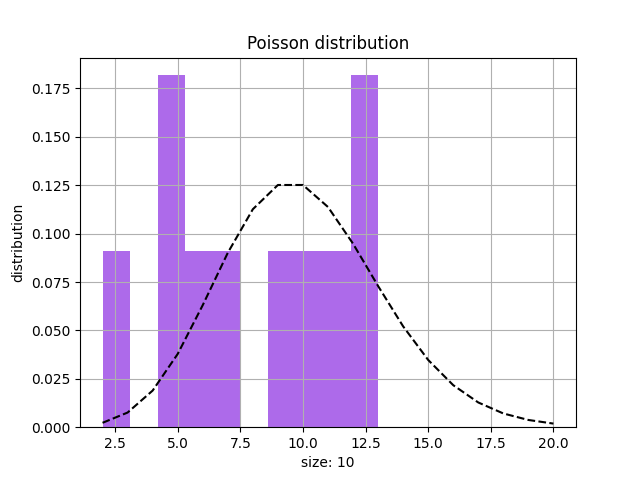
\includegraphics[height = 0.25\textheight, width = 0.31\textwidth]{Poisson_10.png}
        & 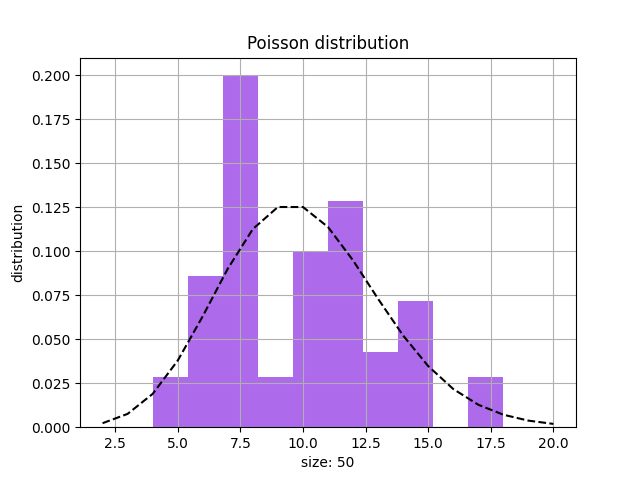
\includegraphics[height = 0.25\textheight, width = 0.31\textwidth]{Poisson_50.png}
        & 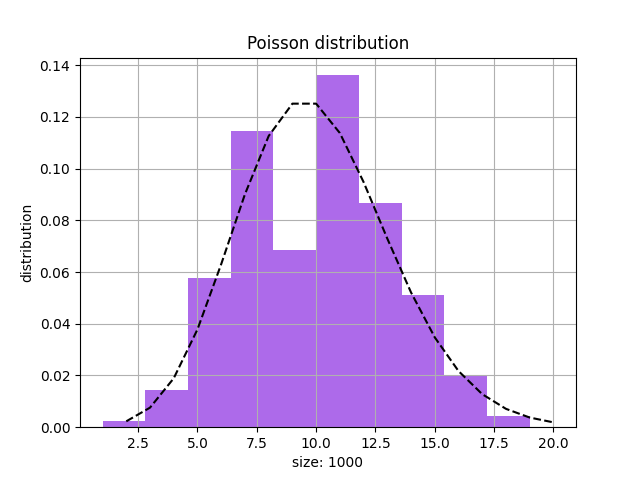
\includegraphics[height = 0.25\textheight, width = 0.31\textwidth]{Poisson_1000.png}
    \end{tabular}
    \caption{Распределение Пуассона\eqref{poisson}}
    \label{fig:poisson}
\end{figure}

\begin{figure}[H]
    \centering
    \begin{tabular}{c c c}
        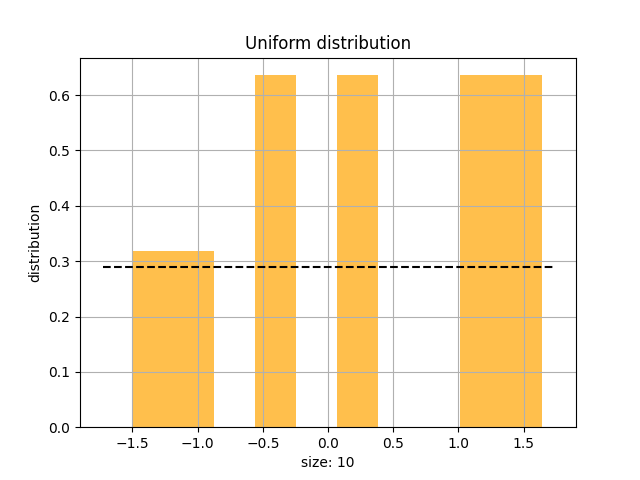
\includegraphics[height = 0.25\textheight, width = 0.31\textwidth]{Uniform_10.png}
        & 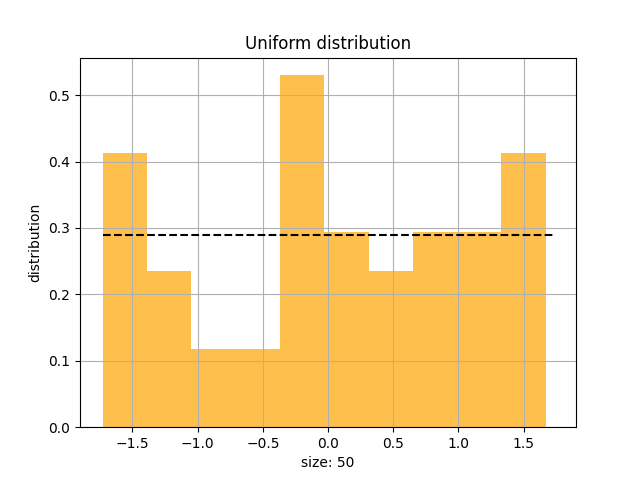
\includegraphics[height = 0.25\textheight, width = 0.31\textwidth]{Uniform_50.png}
        & 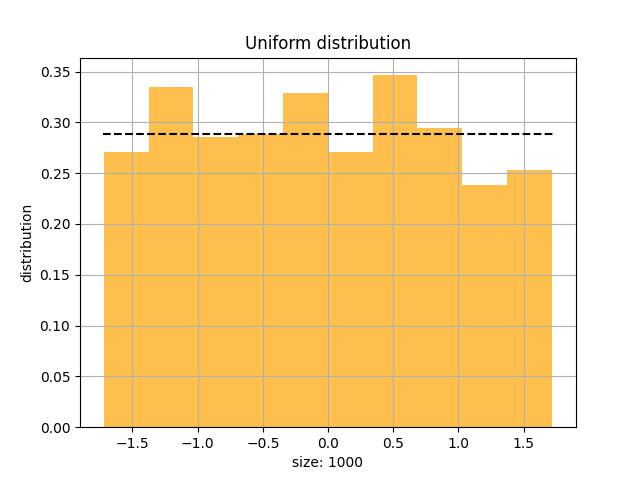
\includegraphics[height = 0.25\textheight, width = 0.31\textwidth]{Uniform_1000.png}
    \end{tabular}
    \caption{Равномерное распределение \eqref{uniform}}
    \label{fig:uniform}
\end{figure}

\section{Обсуждение}
Анализ результатов демонстрирует следующую закономерность для всех распределений: чем больше выборка из распределения, тем больше соответсвует гистограмма распределения графику плотности его распределения. То есть для определения характера распределения величины стоит рассматривать выборки больших размеров.При сравнении гистаграмм распределений между собой можно выделить особенность, что форма гистограмм нормального распределения, распределения Коши, Лапласа плохо отличимы между собой, тем более при маленьком размере выборки. Для этих распределений характерно относительное совпадение пика гистограммы с пиком графика плотности соответсвующего распределения. Также большая часть распределений различается по высоте пиковой точки и по степени близости прохождения ветвек графиков плотностей распределения к ассимптоте и оси симметрии, не считая равномерного распределения.

Стоит отметить, что распределение Пуассона является более широким, что можно выделить, как отличительную черту распределения. Аналогично для равномерного распределения характерно наличие столбцов более или менее однородной высоты. Касательно распределения Коши можно сказать, что высота пиковой точки гистограммы много меньше высоты пиковой точки графика распределения.

На гистограммах наблюдаются всплески, явно превыщающие исходное значение плотности распределения в заданной точке. Но они стихают по мере увеличения размеров выборки.

\end{document}
